\documentclass{standalone}
%
\usepackage{tikz}
\usetikzlibrary{backgrounds, arrows.meta, shapes.callouts}
\usepackage{xcolor}
%
\definecolor{space}{HTML}{1F2C4E}
\definecolor{earth}{HTML}{0089FA}
\definecolor{mars}{HTML}{DC7B4E}
\definecolor{dida}{HTML}{FFDE00}
\definecolor{title}{HTML}{FBA706}
%
\usepackage{fontspec}
\setmainfont{Open Dyslexic}
%
\title{Il motore a curvatura}
\begin{document}
	\tikzset{
		partial ellipse/.style args = {#1:#2:#3}{insert path={+ (#1:#3) arc (#1:#2:#3)}},
		notice/.style  = { draw, ellipse callout, callout relative pointer={#1} },
	}
	\begin{tikzpicture}[background rectangle/.style={fill=white},show background rectangle,>={[inset=0,angle'=27]Stealth}]
		%title
		\draw [black,ultra thick,fill=title] (0,9.8) rectangle (30,16.8);
		\node at (15,14.8) {\textcolor{black}{\fontsize{90}{91}\selectfont Il motore}};
		\node at (15,11.8) {\textcolor{black}{\fontsize{90}{91}\selectfont a curvatura}};
		%
		\begin{scope}[shift={(0,5)}]
			\draw [ultra thick, fill=earth] (20.5,4) rectangle (25.5,-4);
			\node at (23,0) {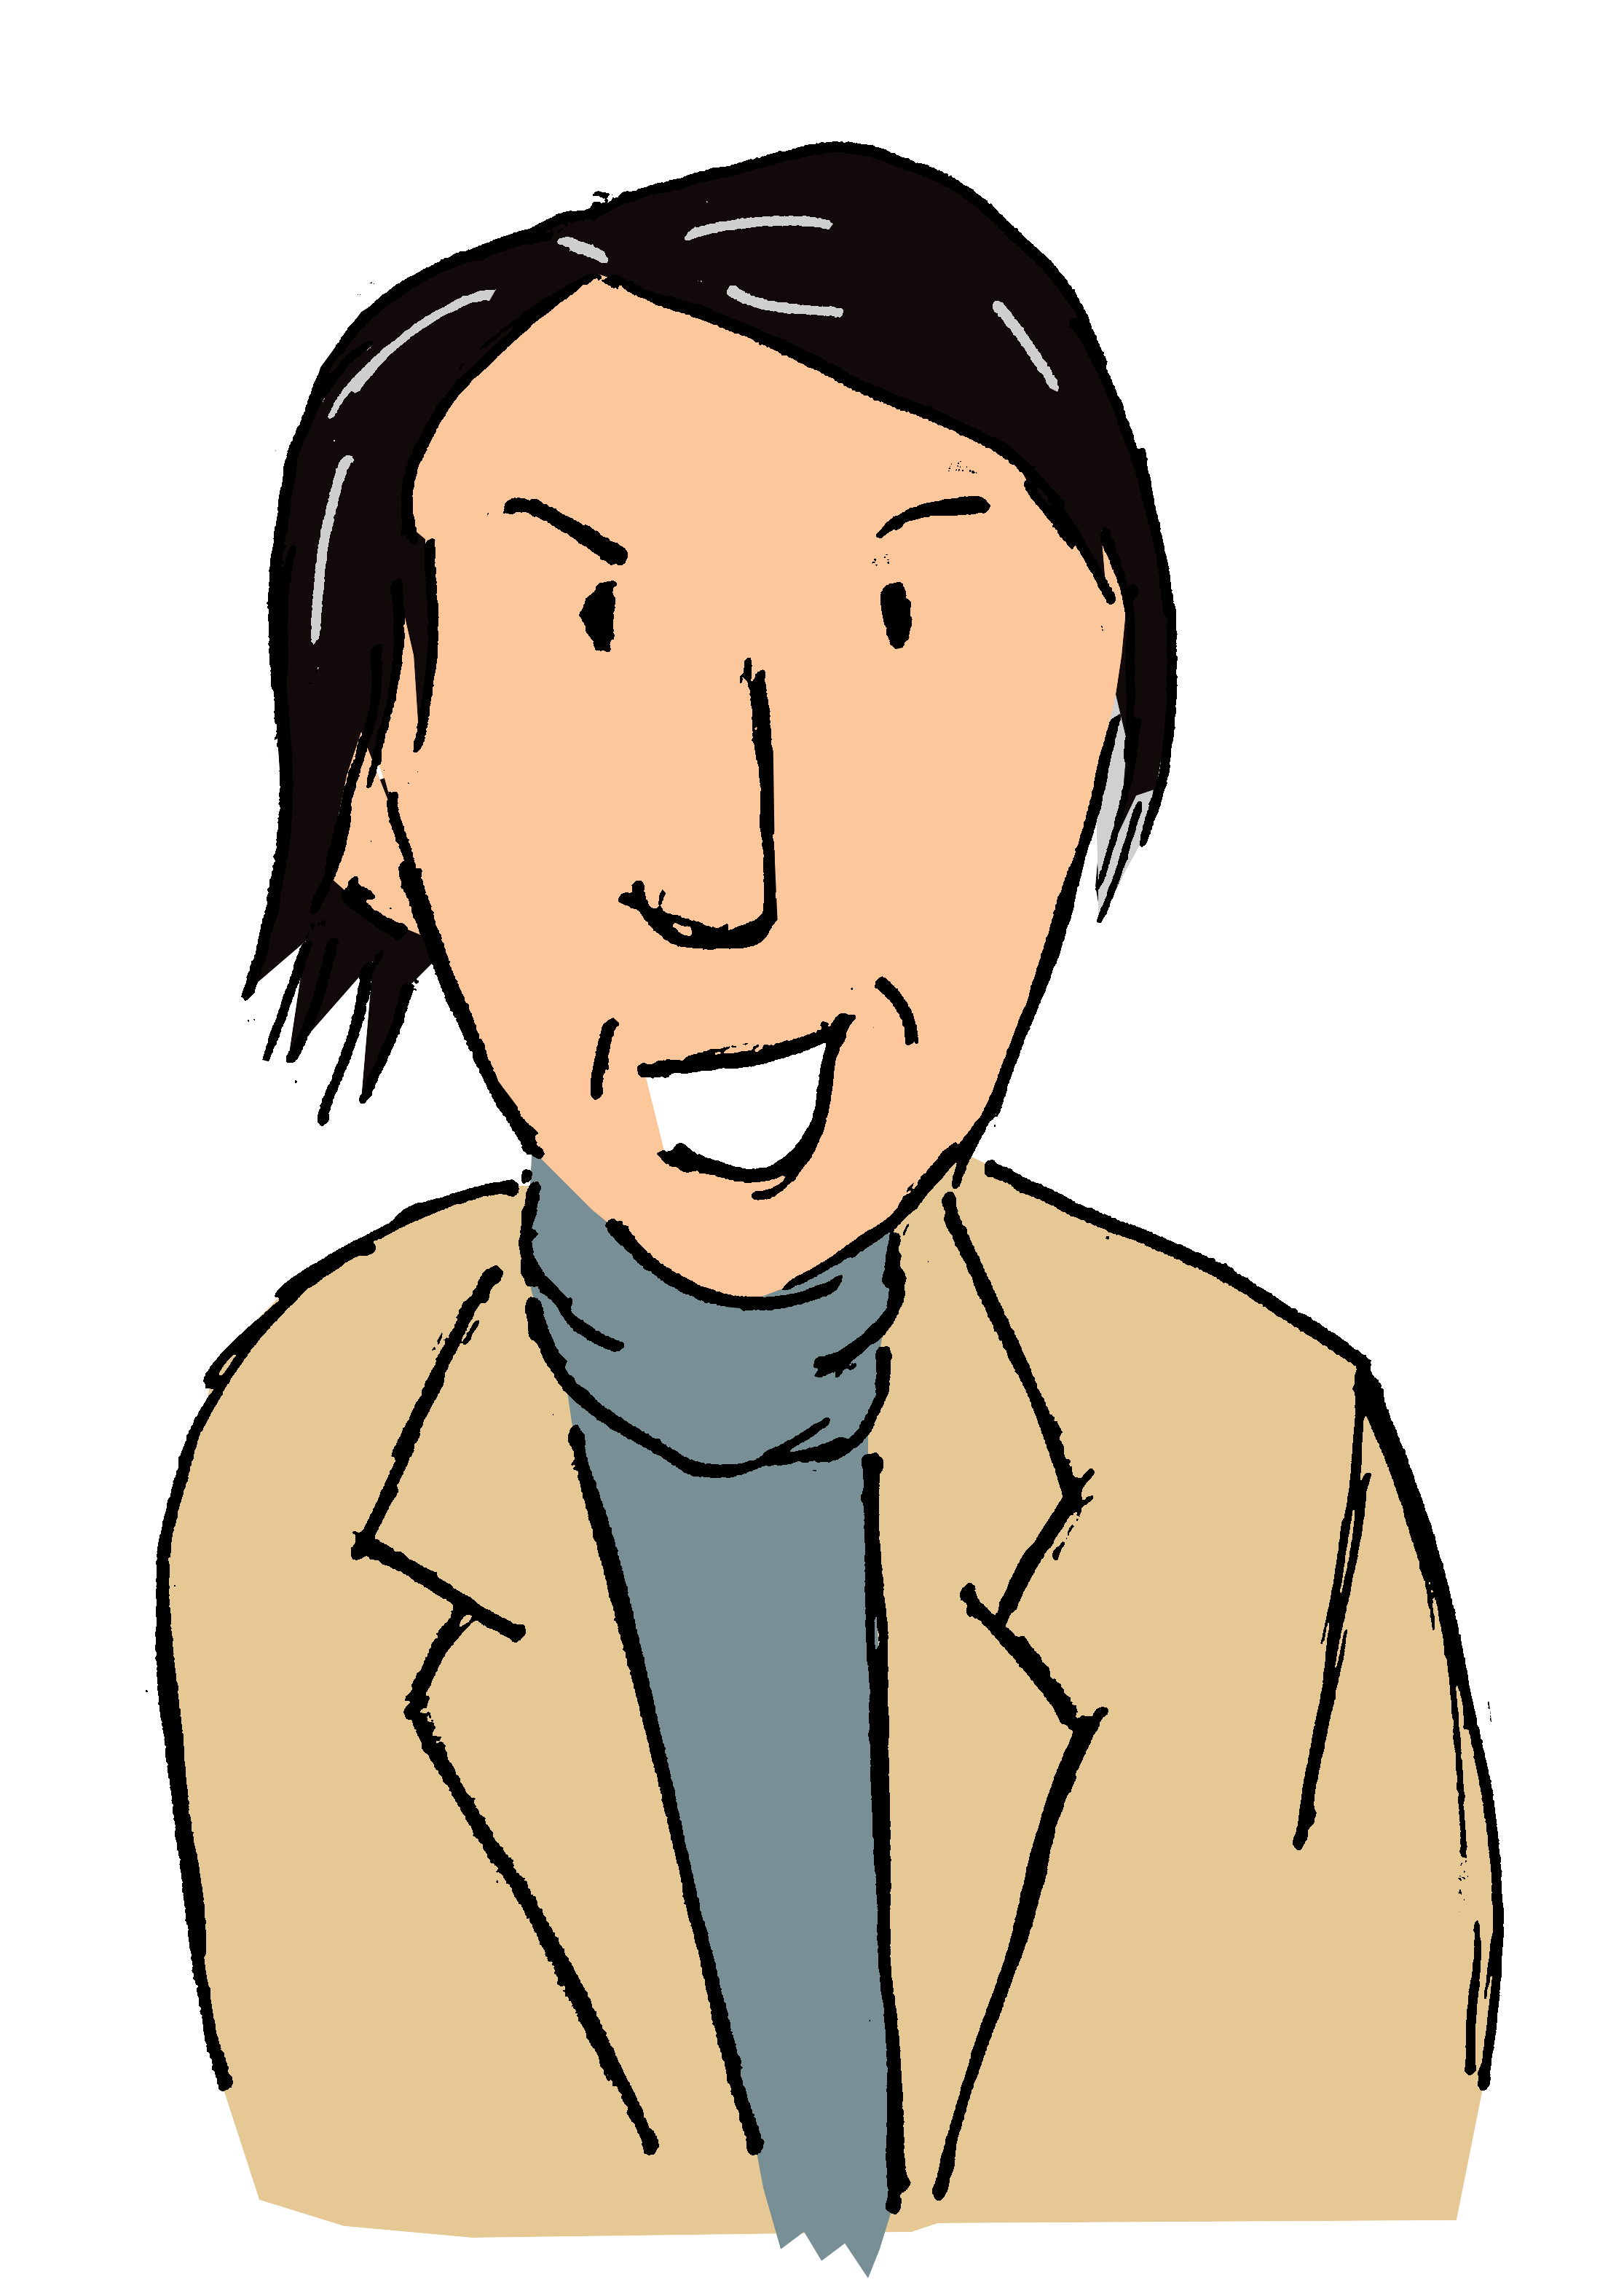
\includegraphics[width=5cm]{carl_sagan}};
			\node (example-textwidth-2) [notice={(3,0.5)}, ultra thick, right, align=center, text width=12cm, color=black, fill=white, font=\fontsize{23pt}{24pt}\selectfont] at (1,-1) {Benvenuti! Sono Carl Sagan e oggi vi racconterò qualcosa su uno dei dispositivi più noti di \emph{Star Trek}: il motore a curvatura!};
		\end{scope}
		%
		\begin{scope}[shift={(16,-11.5)}]
			%
			\draw [fill=space, ultra thick] (-13,9) rectangle (13,-5);
			%
			\draw [color=white] (-0.1,-2.9) to[out=90,in=275] (-0.9,8.3);
			\draw [color=white] (-0.6,-2.7) to[out=98,in=300] (-5.1,7.8);
			\draw [color=white] (-1.1,-2.7) to[out=100,in=314] (-8.7,6.7);
			\draw [color=white] (-1.3,-2.4) to[out=120,in=325] (-5.9,1.9) to[out=148,in=335] (-11.2,4.9);
			\draw [color=white] (-1.6,-2.4) to[out=130,in=330] (-4.9,0.1) to[out=150,in=340] (-12,2.9);
			%
			\draw [color=white] (0.3,-2.9) to[out=81,in=250] (3.5,8.1);
			\draw [color=white] (0.8,-2.6) to[out=76,in=231] (7.4,7.2);
			\draw [color=white] (1.4,-2.5) to[out=65,in=214] (10.5,5.6);
			\draw [color=white] (1.7,-2.4) to[out=75,in=210] (4.85,0.5) to[out=20,in=180] (11.9,2.4);
			%
			\draw (0,-1.8) [color=white,partial ellipse=0:180:2.1 and 1];
			\draw (0,-1.2) [color=white,partial ellipse=0:180:2.8 and 1.3];
			\draw (0,-0.6) [color=white,partial ellipse=0:180:3.5 and 1.6];
			\draw (0,0) [color=white,partial ellipse=0:180:4.2 and 1.8];
			\draw (0,0.3) [color=white,partial ellipse=0:180:4.9 and 2.1];
			%
			\node at (0,0) {\includegraphics[width=5cm,angle=-50]{astronave}};
			%
			\draw [color=white] (-1.6,-2.4) to[out=150,in=330] (-3.5,-1) to[out=160,in=350] (-10.8,0.7);
			\draw [color=white] (-1.3,-2.6) to[out=165,in=330] (-2.9,-1.4) to[out=165,in=360] (-7.8,-1);
			\draw [color=white] (-1,-2.7) to[out=130,in=330] (-2,-1.6) to[out=160,in=30] (-4.6,-1.9);
			\draw [color=white] (-0.5,-2.85) to[out=90,in=350] (-1,-1.8) to[out=160,in=40] (-1.8,-2.25);
			%
			\draw [color=white] (1.5,-2.5) to[out=80,in=214] (3.5,-1) to[out=20,in=180] (9,-0.5);
			\draw [color=white] (0.65,-2.8) to[out=80,in=214] (1.7,-1.7) to[out=20,in=170] (5.2,-1.8);
			\draw [color=white] (0.1,-2.9) to [out=88,in=250] (0.3,-1.8) to[out=20,in=140] (1,-2.3);
			%
			\draw (0,-1.8) [color=white,partial ellipse=180:360:2.1 and 1];
			\draw (0,-1.2) [color=white,partial ellipse=180:360:2.8 and 1.3];
			\draw (0,-0.6) [color=white,partial ellipse=180:360:3.5 and 1.6];
			\draw (0,0) [color=white,partial ellipse=180:360:4.2 and 1.8];
			\draw (0,0.3) [color=white,partial ellipse=180:360:4.9 and 2.1];
			\draw [color=white] (0,0.6) ellipse (5.6cm and 2.4cm);
			\draw [color=white] (0,0.9) ellipse (6.3cm and 2.7cm);
			\draw [color=white] (0,1.2) ellipse (7cm and 3cm);
			\draw [color=white] (0,1.5) ellipse (7.7cm and 3.3cm);
			\draw [color=white] (0,1.8) ellipse (8.5cm and 3.7cm);
			\draw [color=white] (0,2.1) ellipse (9.3cm and 4.1cm);
			\draw [color=white] (0,2.4) ellipse (10.2cm and 4.5cm);
			\draw [color=white] (0,2.7) ellipse (11.1cm and 4.9cm);
			\draw [color=white] (0,3) ellipse (12cm and 5.3cm);
			%dida
			\draw [black,thick,fill=dida] (-2,12) rectangle (14,8);
			\node (example-textwidth-2) [right, align=left, text width=15cm, color=black, font=\fontsize{23pt}{24pt}\selectfont] at (-1.5,10) {Partiamo da un fatto noto: tutti gli oggetti nell'universo deformano lo spaziotempo. Incluse le navicelle spaziali.};
			%
			\draw [black,thick,fill=dida] (-16,-4) rectangle (-3,-6.5);
			\node (example-textwidth-2) [right, align=left, text width=15cm, color=black, font=\fontsize{23pt}{24pt}\selectfont] at (-15.5,-5.25) {Questa deformazione viene chiamata \textbf{curvatura}.};
		\end{scope}
		%
		\begin{scope}[shift={(0,-27)}]
			\draw[fill=space,ultra thick] (0.5,7.5) rectangle (29,-5.5);
			\begin{scope}[shift={(-6,0)}]
				\begin{scope}[rotate around={10:(12.8,0)}]
					\draw (15,0) [color=white,partial ellipse=0:360:2.2 and 1.2];
					\draw (15,0) [color=white,partial ellipse=180:380:2.5 and 1.5];
				\end{scope}
				\begin{scope}[rotate around={14:(12.8,0)}]
					\draw [color=white] (10,-2.5) -- (20,-2.5);
				\end{scope}
				\draw (15,0) [color=white,partial ellipse=180:110:2.2 and 4];
				\draw (15,0) [color=white,partial ellipse=160:40:2.5 and 4.3];
				\draw [color=white] (11.5,0) to[out=0,in=260] (12.65,1.5);
				\draw [color=white] (16.9,2.8) to[out=290,in=180] (18.5,2);
				\draw [color=white] (17.15,0.7) -- (17.2,0.05);
				\draw [color=white] (17.45,-1.4) -- (17,-4) to[out=240,in=-45] (14.8,-2.1);
				%
				\draw[<-,ultra thick,color=white] (15.5,0.5) -- (22,-1);
				\node (example-textwidth-2) [right, align=left, text width=8cm, color=white, font=\fontsize{23pt}{24pt}\selectfont] at (22,-1) {zona di competenza della navicella};
				%
				\draw [<-,ultra thick,color=white] (14.5,2.5) -- (11,5);
				\draw [<-,ultra thick,color=white] (16.5,-3.5) -- (10.8,5);
				\node (example-textwidth-2) [right, align=left, text width=15cm, color=white, font=\fontsize{23pt}{24pt}\selectfont] at (8,5.5) {deformazioni spaziotemporali};
			\end{scope}
			\draw [black,thick,fill=dida] (16.5,9.5) rectangle (29.5,0.5);
			\node (example-textwidth-2) [right, align=left, text width=12cm, color=black, font=\fontsize{23pt}{24pt}\selectfont] at (17,5) {Ed è questo il concetto scientifico dietro il motore a curvatura di Star Trek, solo che all'epoca un'idea del genere non era per nulla venuta in mente ai fisici, fino a che nel 1994 Miguel Alcubierre non porpose qualcosa del genere.};
		\end{scope}
		%
		\begin{scope}[shift={(0,-35.5)}]
			\draw [fill=space,ultra thick] (0.5,2) rectangle (29.5,-12);
			%dida up
			\draw [fill=dida,thick] (1,2.5) rectangle (29,-2.5);
			\node (example-textwidth-2) [right, align=left, text width=27cm, color=black, font=\fontsize{23pt}{24pt}\selectfont] at (2,0) {La sua "guida a curvatura" prevede la deformazione dello spaziotempo intorno all'astronave: si generano due zone, una con curvatura positiva con conseguente espansione dello spaziotempo locale, e un'altra con curvatura negativa, e contrazione dello spaziotempo.};
			%
			\node at (25,-8) {\includegraphics[width=5cm,angle=-50]{astronave}};
			\node (example-textwidth-2) [notice={(3,0.5)}, ultra thick, right, align=center, text width=6cm, color=black, fill=white, font=\fontsize{23pt}{24pt}\selectfont] at (12,-8) {Vieni da me!};
			\draw [fill=mars,ultra thick] (5,-8) circle (3 cm);
			\draw [->,ultra thick,color=white] (8.5,-8) -- (10,-8);
		\end{scope}
		%
		\begin{scope}[shift={(0,-50)}]
			\draw [fill=dida,thick] (1,2.2) rectangle (29,-2.2);
			\node (example-textwidth-2) [right, align=left, text width=27cm, color=black, font=\fontsize{23pt}{24pt}\selectfont] at (1.6,0) {In questo modo è possibile avvicinare il punto di arrivo e, soprattutto, a muoversi più veloce della luce è lo spaziotempo, cosa permessa dalla relatività generale, mentre l'astronave resta "ferma".};
			\node at (25,-8) {\includegraphics[width=7cm]{miguel_alcubierre}};
			\node (example-textwidth-2) [notice={(3,0.5)}, ultra thick, right, align=center, text width=12cm, color=black, fill=white, font=\fontsize{23pt}{24pt}\selectfont] at (1,-8) {Mi sono ispirato proprio a Star Trek per sviluppare il modello matematico dietro questo motore a curvatura!};
		\end{scope}
		%
		\begin{scope}[shift={(0,-64)}]
			\node at (27,0) () {
\includegraphics[width=3.7cm]{licenza}};
			\node at (18,-0.1) {\textcolor{black}{\fontsize{14}{15}\selectfont Testo e illustrazioni: @ulaulaman - Gianluigi Filippelli}};
		\end{scope}
	\end{tikzpicture}
%
\end{document}
